
After the discovery of the new boson, the next most important topic is to examine its properties. 
The SM Higgs has $J^{CP} = 0^{++}$ where J is spin, C is charge, and P is parity
and those quantum numbers are conserved in interactions. In some BSM models such 
as SUSY, the Higgs sector can be expanded to CP-odd scalar or psedoscalar particles, 
or a mixture of them that leads to CP-violation.
Spin-1 model is excluded because the new boson decays to two massless bosons, 
\textit{i.e.}, photons, which is not possible for a massive spin-1 resonance 
due to Yang's theorem~\cite{PhysRev.77.242}. 
So, we intend to study alternative spin-0 and spin-2 models.   


In the reference \cite{Bolognesi:2012mm}, phenomenological studies of the scattering 
amplitudes of SM Higgs or exotic boson wth different spin-parity natures are performed.  
The study shows that \hww\ channel has a good 
sensitivity to distinguish the SM Higgs from a spin-2 resonance that couples to 
the \ww\ through a minial couplings. This model is denoted as $2_{min}^+$
and the SM Higgs boson is denoted as $0^+$. 

This section descirbes the spin-2 model, the helicity argument 
of \ww\ decay, method of study and the result. 

\section{Introduction} 

A general form of scattering amplitude of a spin-two resonance that decays to two vector 
bosons is given in~\cite{Bolognesi:2012mm}. The mininal coupling senario 
where only two couplings are non-zero gives the scattering amplitude 
\begin{eqnarray} 
A(X \rightarrow V_1V_2)
&=& 
\frac{1}{\Lambda^2}  
\left[ 
2 g_2^{(2)} t_{\mu\nu} \frac{q_\alpha q_\beta}{\Lambda^2} 
f^{(1)\mu\alpha*} f^{(2)\nu\beta*} 
+ 
2 m_V^2 g_5^{(2)} t_{\mu\nu} 
\epsilon^{\mu*}_1 \epsilon^{\nu*}_2 
\right] 
\end{eqnarray} 
where $\Lambda$ is the energy scale where new physics occur, 
$g_2^{(2),(5)}$ is the coupling constant to be measured, 
$t_{\mu\nu}$ is the wave function of X given by a sysmetric tracless tensor, 
$q_{\alpha}$ is the 4-momentum of X, 
$f^{(i)\mu\alpha}$ is the field strength tensor given by 
    $\epsilon_i^\mu q_i^\alpha - \epsilon_i^\alpha q_i^\mu$, 
$m_V$ is the mass of gauge boson, and 
$\epsilon_i^{\mu}$ is the polarization vector of the gauge boson i.
This is the model similar to minimal coupling Kaluza-Klein graviton with spin-2~\cite{}. 

Because of different spin structure of SM Higgs boson and the $2_{min}^+$ model, 
the kinematics of the two bosons that decay from the resonance is different. 
A simple argument can be given based on the helicity conservation. 
This can be expressed using Wigner's d-matrix~\cite{}, $D^{j}_{m'm}$, where 
j is the total spin of the system, and  m' and m are the z-component of spin 
in the initial resonance and the final boson system. 
Let's assume that the beam axis is long the z axis and consider 
decay of gauge bosons in the rest frame of SM Higgs boson. 
The decay plane(the line that the two bosons are in when they fly away each other) 
of the two bosons do not have any preference because SM Higgs boson has spin-0. 
The Wigner's d-matrix in this case is $D_{00}^{0} = 1$. 
On the other hand, in case of the $2_{min}^+$ model, in order for the 
total helicity to be 0 in the boson system, the bosons   
\textcolor{red}{how to proceed for spin-2 case? Is $2_{min}^+$ in $|2,2>$ state?
then, d-function is $\left( \frac{1+\cos \theta}{2} \right)^2$ and this is 
consistent with blue tri-angle in the Phi plot in the middle.} 

The spin-2 sample is generated by JHUGen~\cite{} with matrix element calculation at LO. 
The rest of the simulation for parton showering, hadronization, and underlying events 
is done by PYTHIA~\cite{}. JHUGen generator is validated by generating SM Higgs boson
events and comparing it with anoter generators. 
At the generator level, JHUGen is validated by comparing kinematic distributions 
with the result of MCFM. 
At the reconstruction level, JHUGen+PYTHA is validated by comparing kinematic 
distributions with the result of POWHEG+PYTIHA.
Both comparisons show good agreement. 

\section{Test Method}

\subsubsection{Templates}

In order to discriminate between SM Higgs boson and $2_{min}^+$ model,
we first construct 2-dimensional templates with \mT\ and \mll\ for the signal 
and the background processes in \DF\ 0-jet and 1-jet categories..
We use the same 2-dimensional templates 
as used for the SM Higgs search, which are described in detail in 
section~\ref{sec:shape}. At generator level with no cuts are applied, 
\delphill\ is the variable that separates the two hypotheses most. But, after 
selections are made to suppress backgrounds and the boost of Higgs system 
is taken into account, the separation power is diluted, and \mll\ gives better 
separation power.

\begin{figure}[ht!] 
\centering 
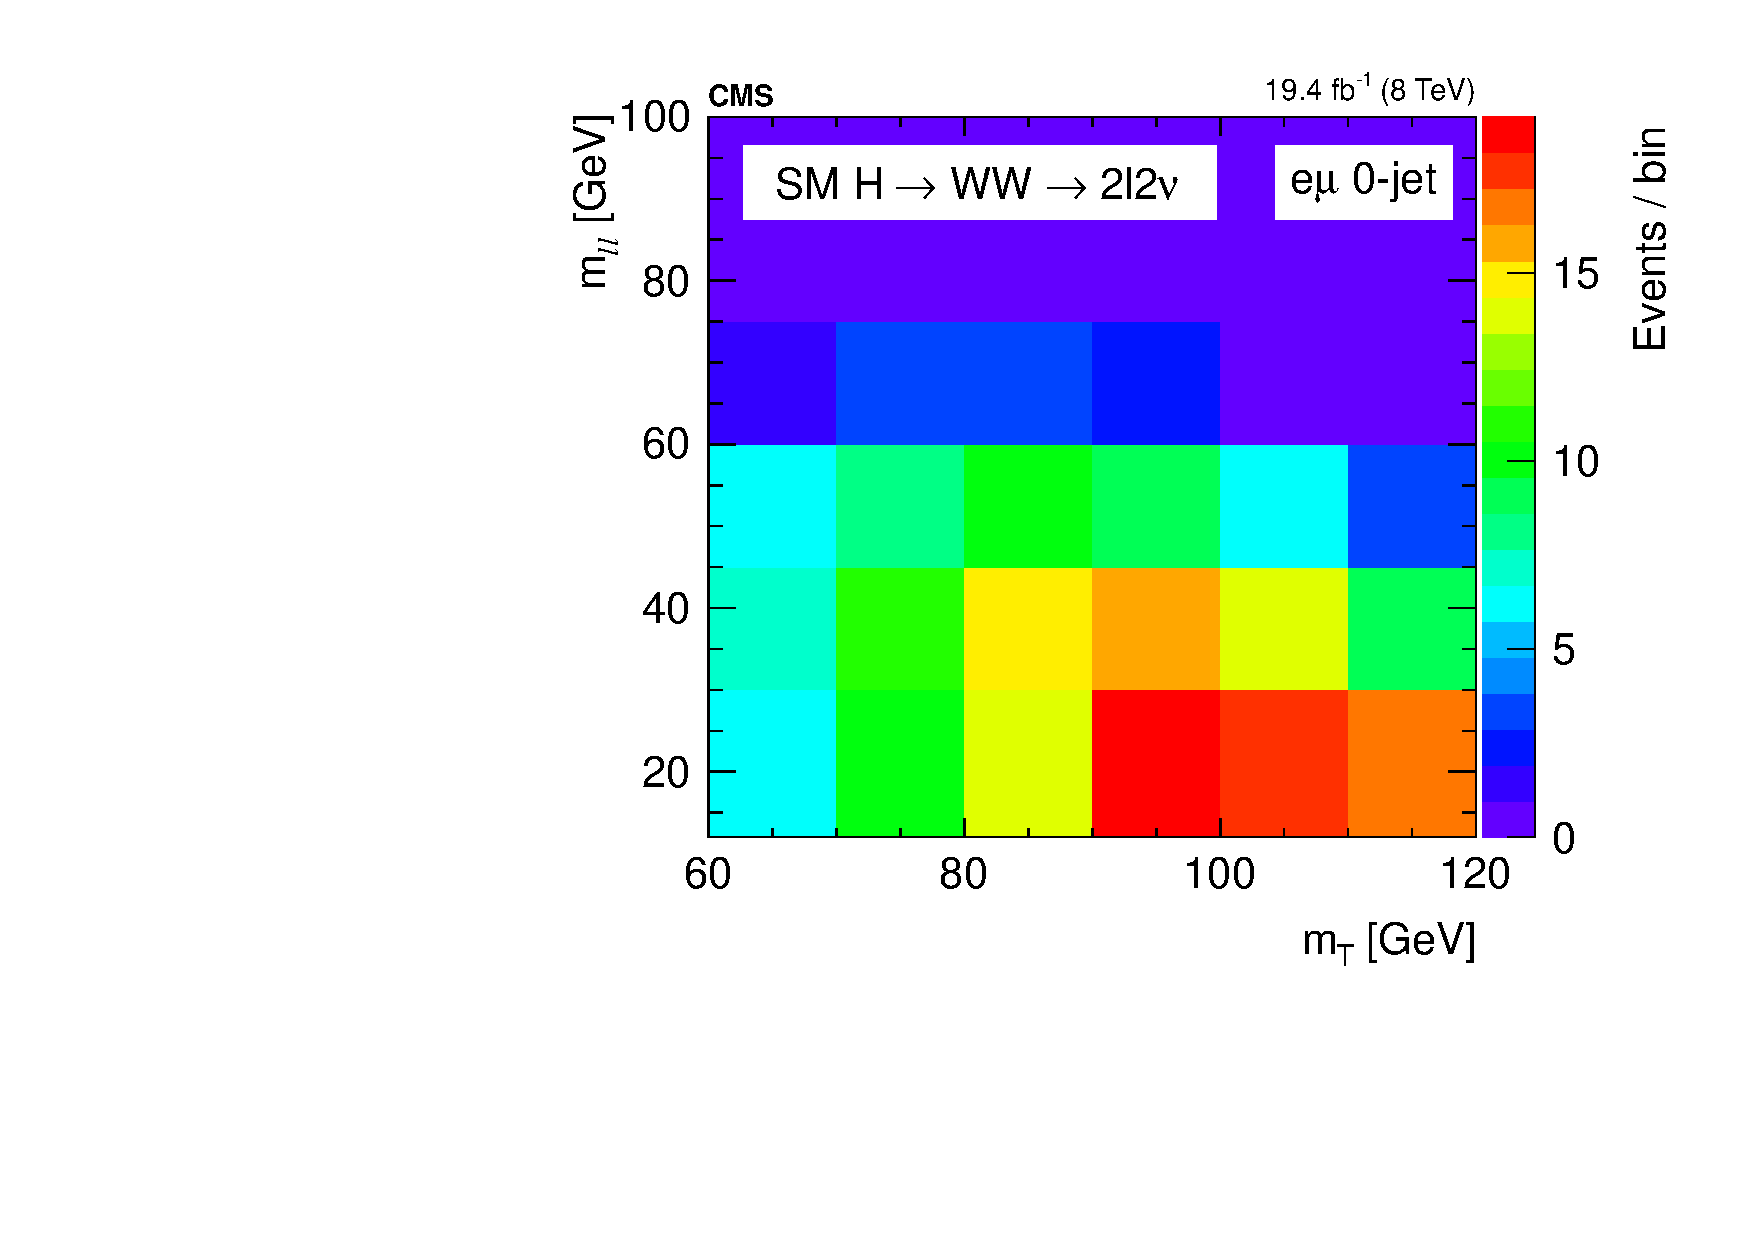
\includegraphics[width=0.45\textwidth]{figures/2d_prefit_0j_125_sig_paper.pdf}
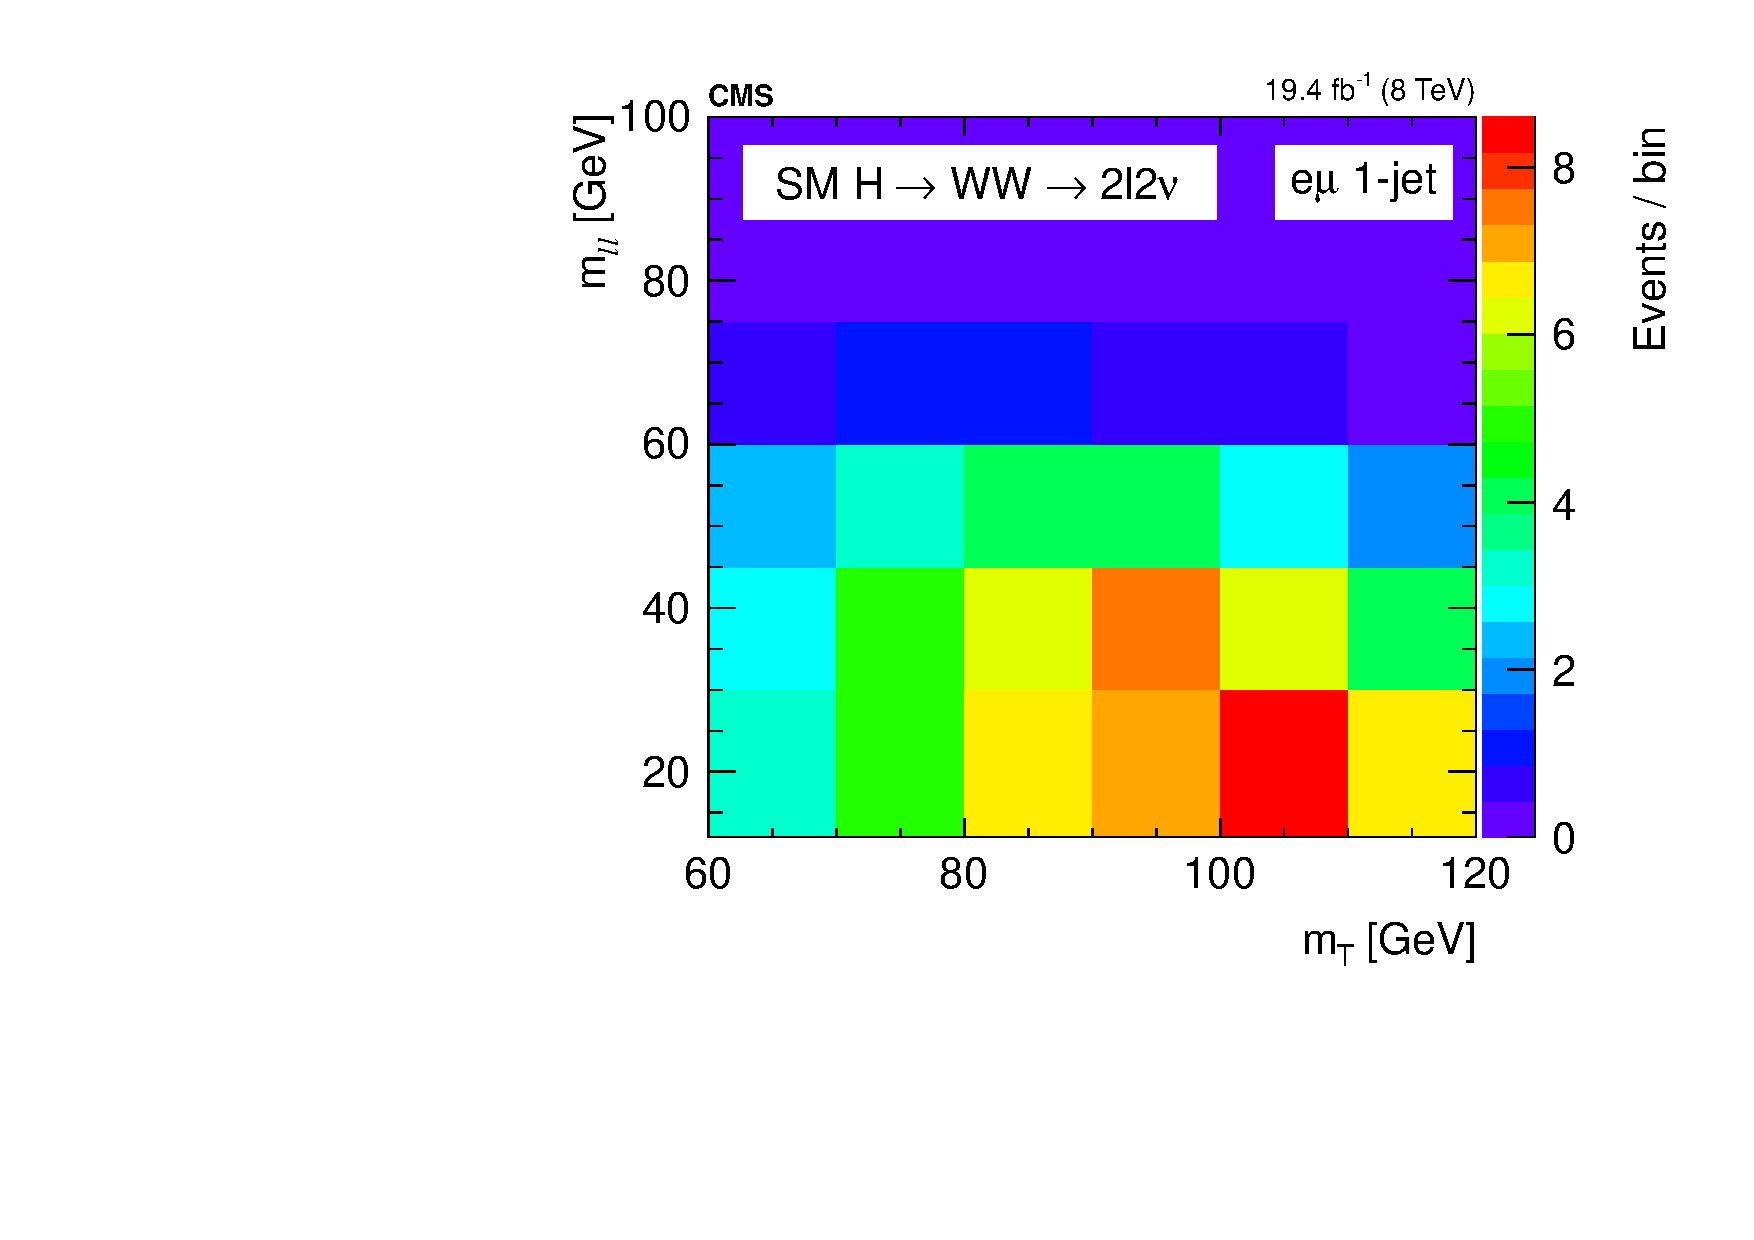
\includegraphics[width=0.45\textwidth]{figures/2d_prefit_1j_125_sig_paper.pdf}
\\
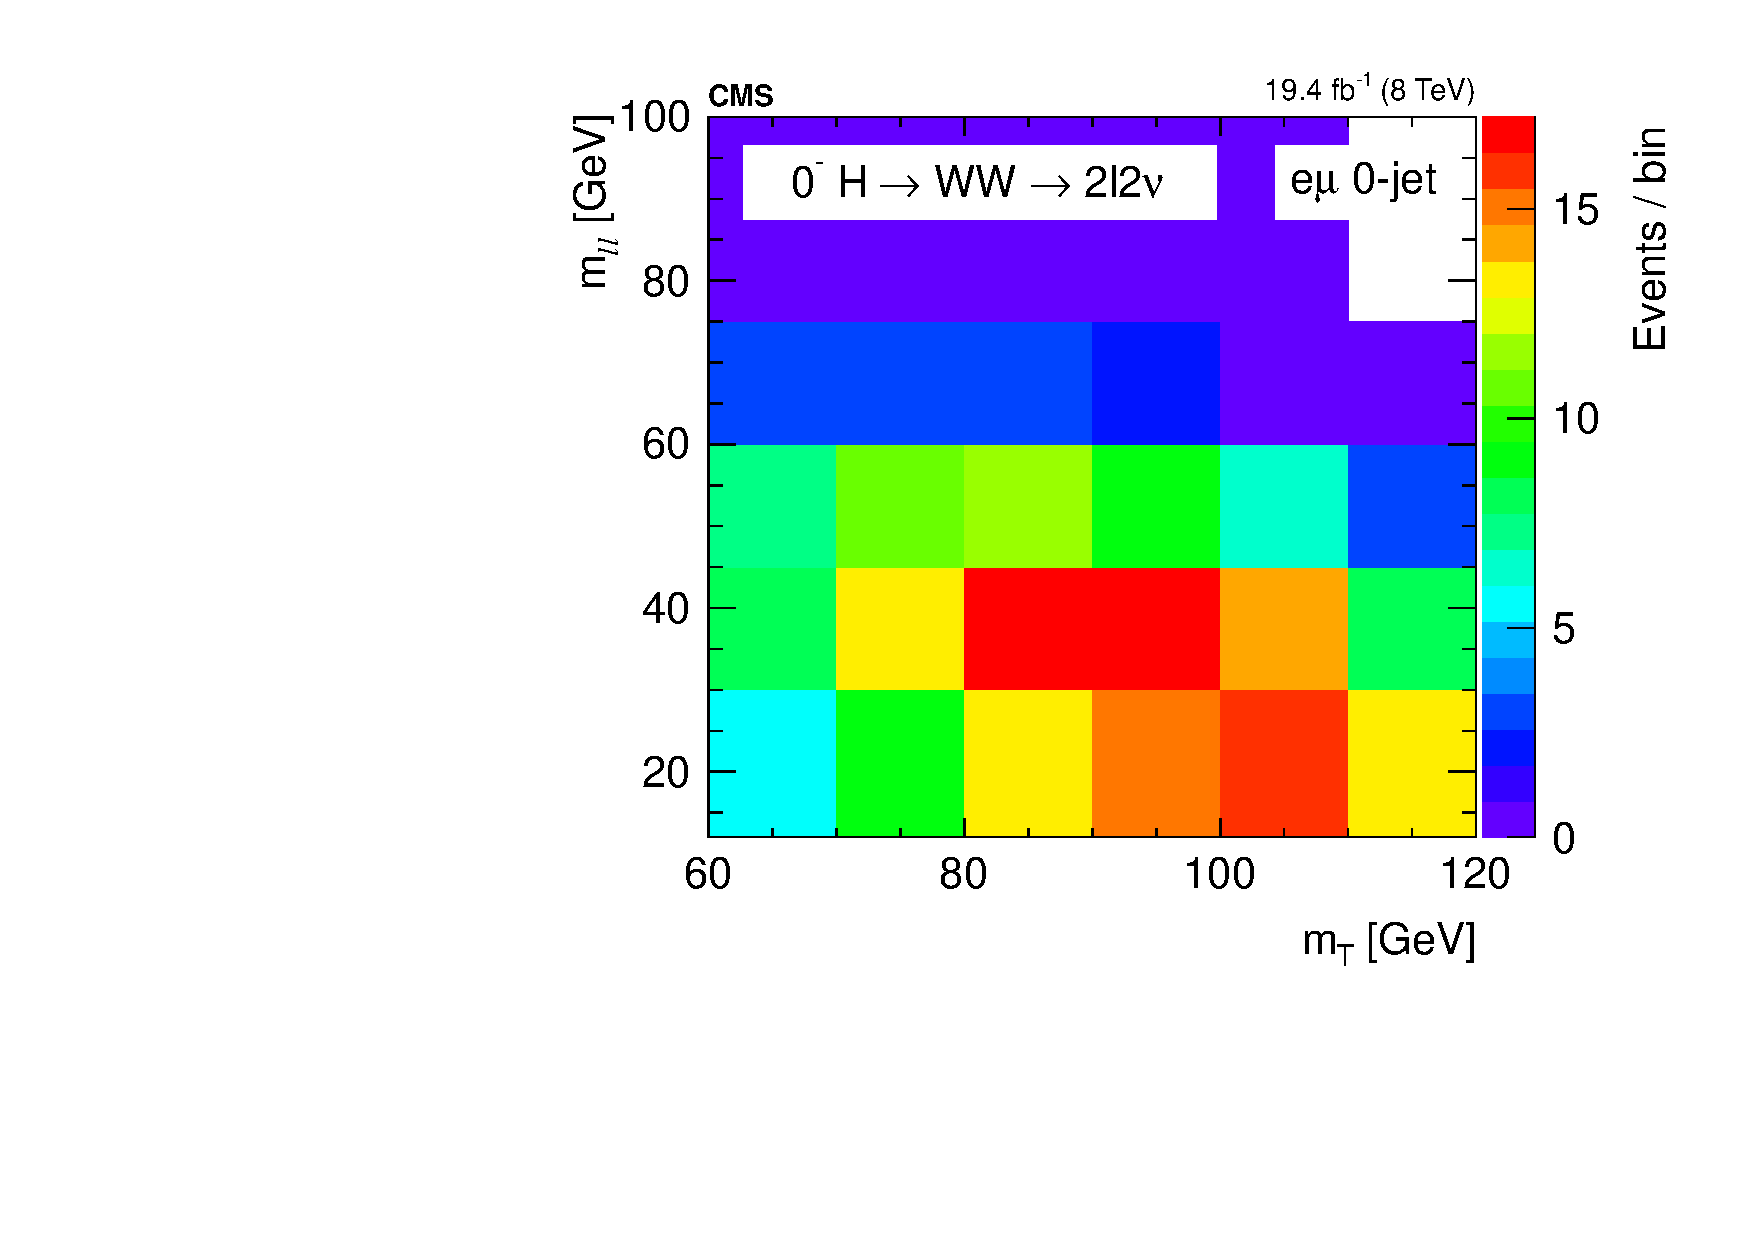
\includegraphics[width=0.45\textwidth]{figures/2d_prefit_0j_125_spin0m_paper.pdf}
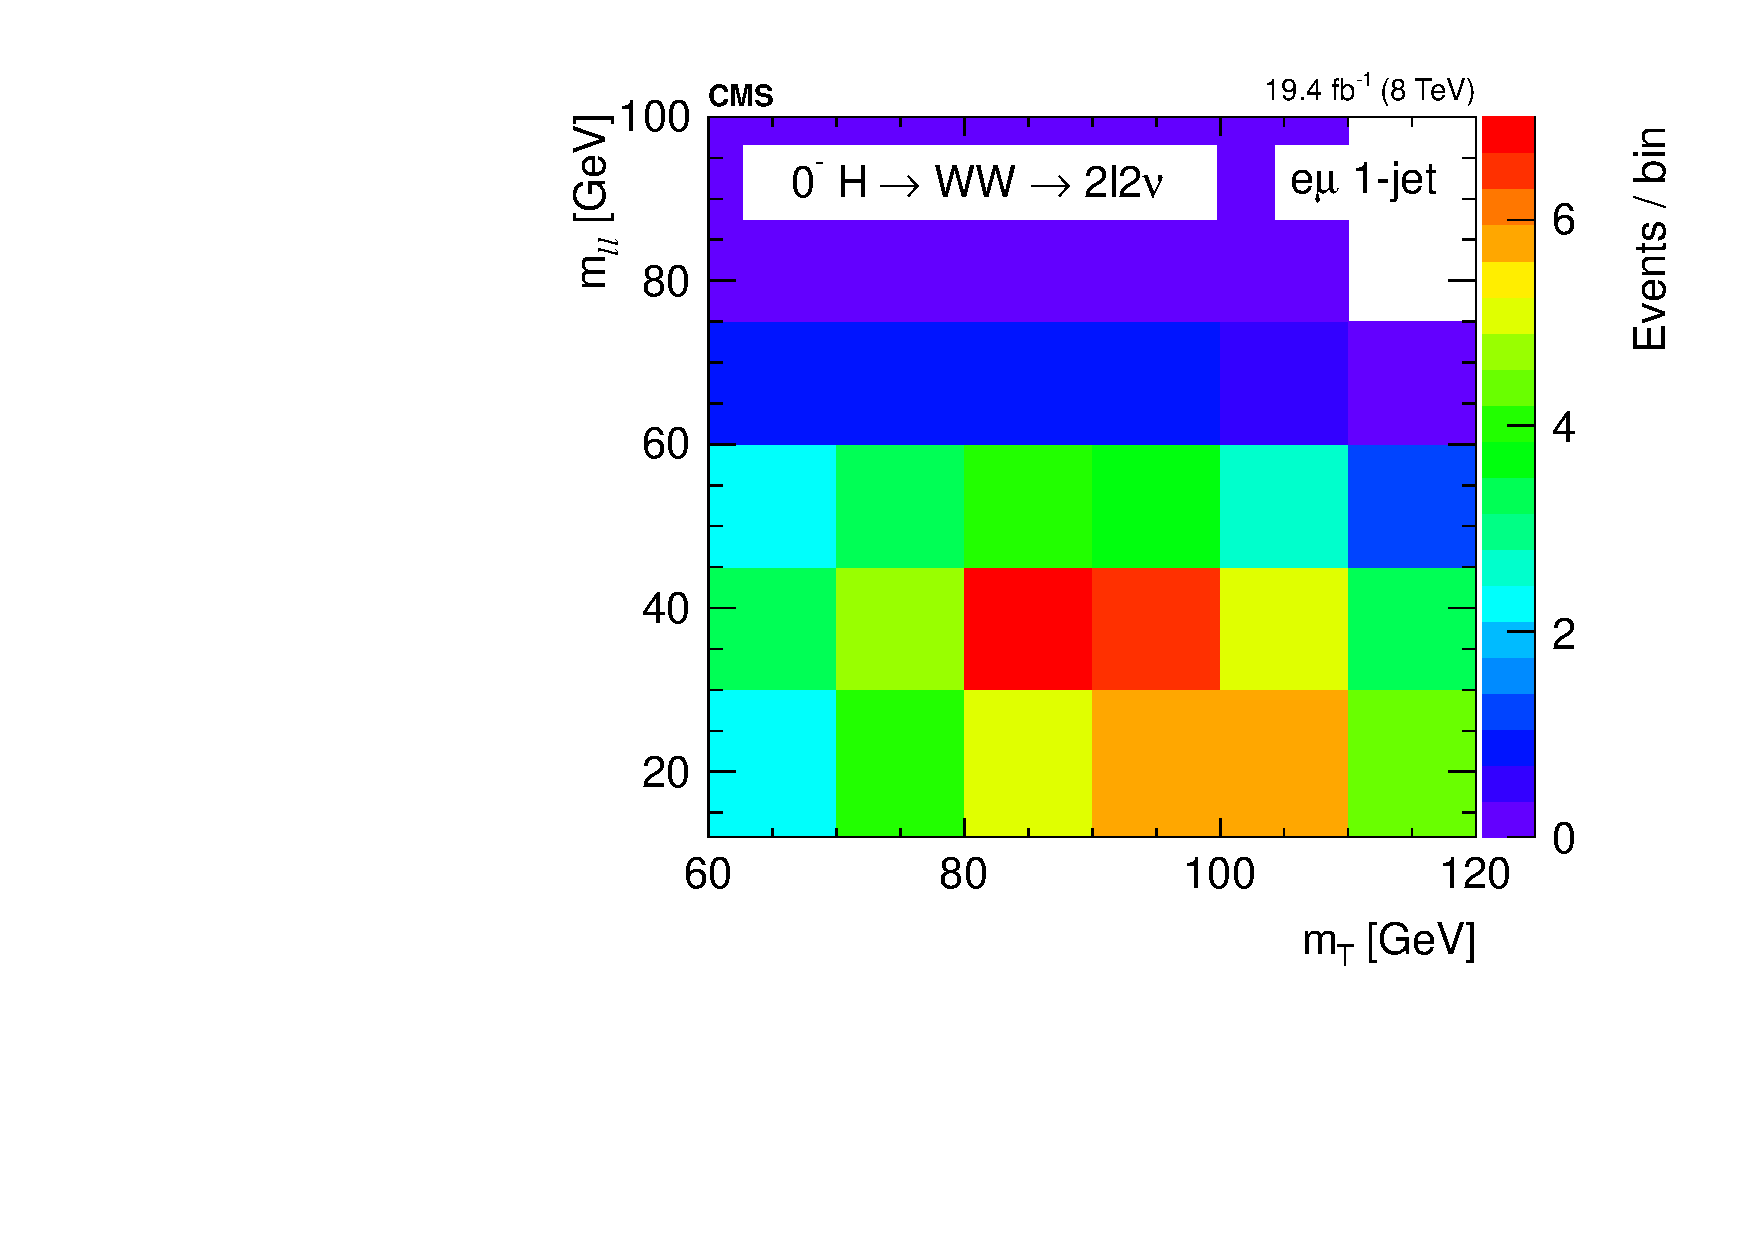
\includegraphics[width=0.45\textwidth]{figures/2d_prefit_1j_125_spin0m_paper.pdf}
\\
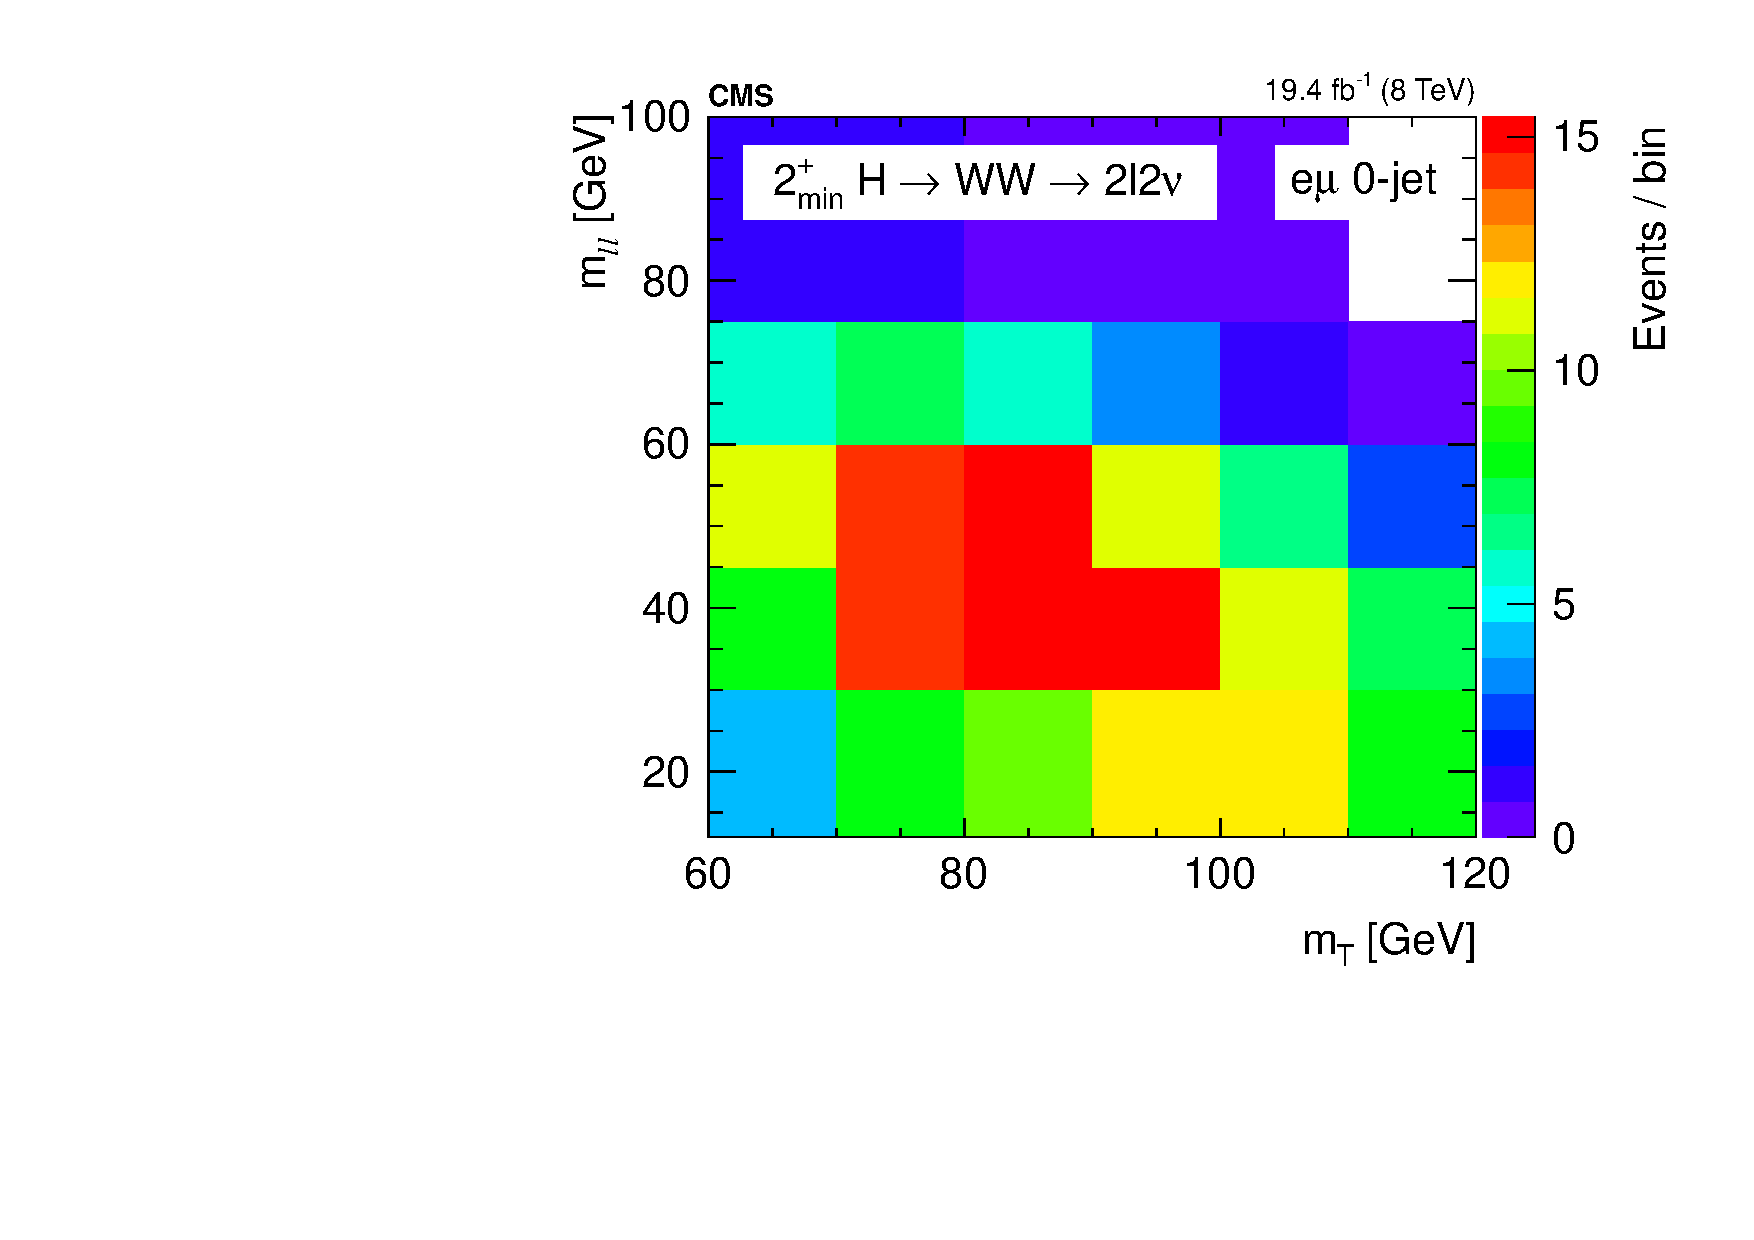
\includegraphics[width=0.45\textwidth]{figures/2d_prefit_0j_125_spin2_paper.pdf}
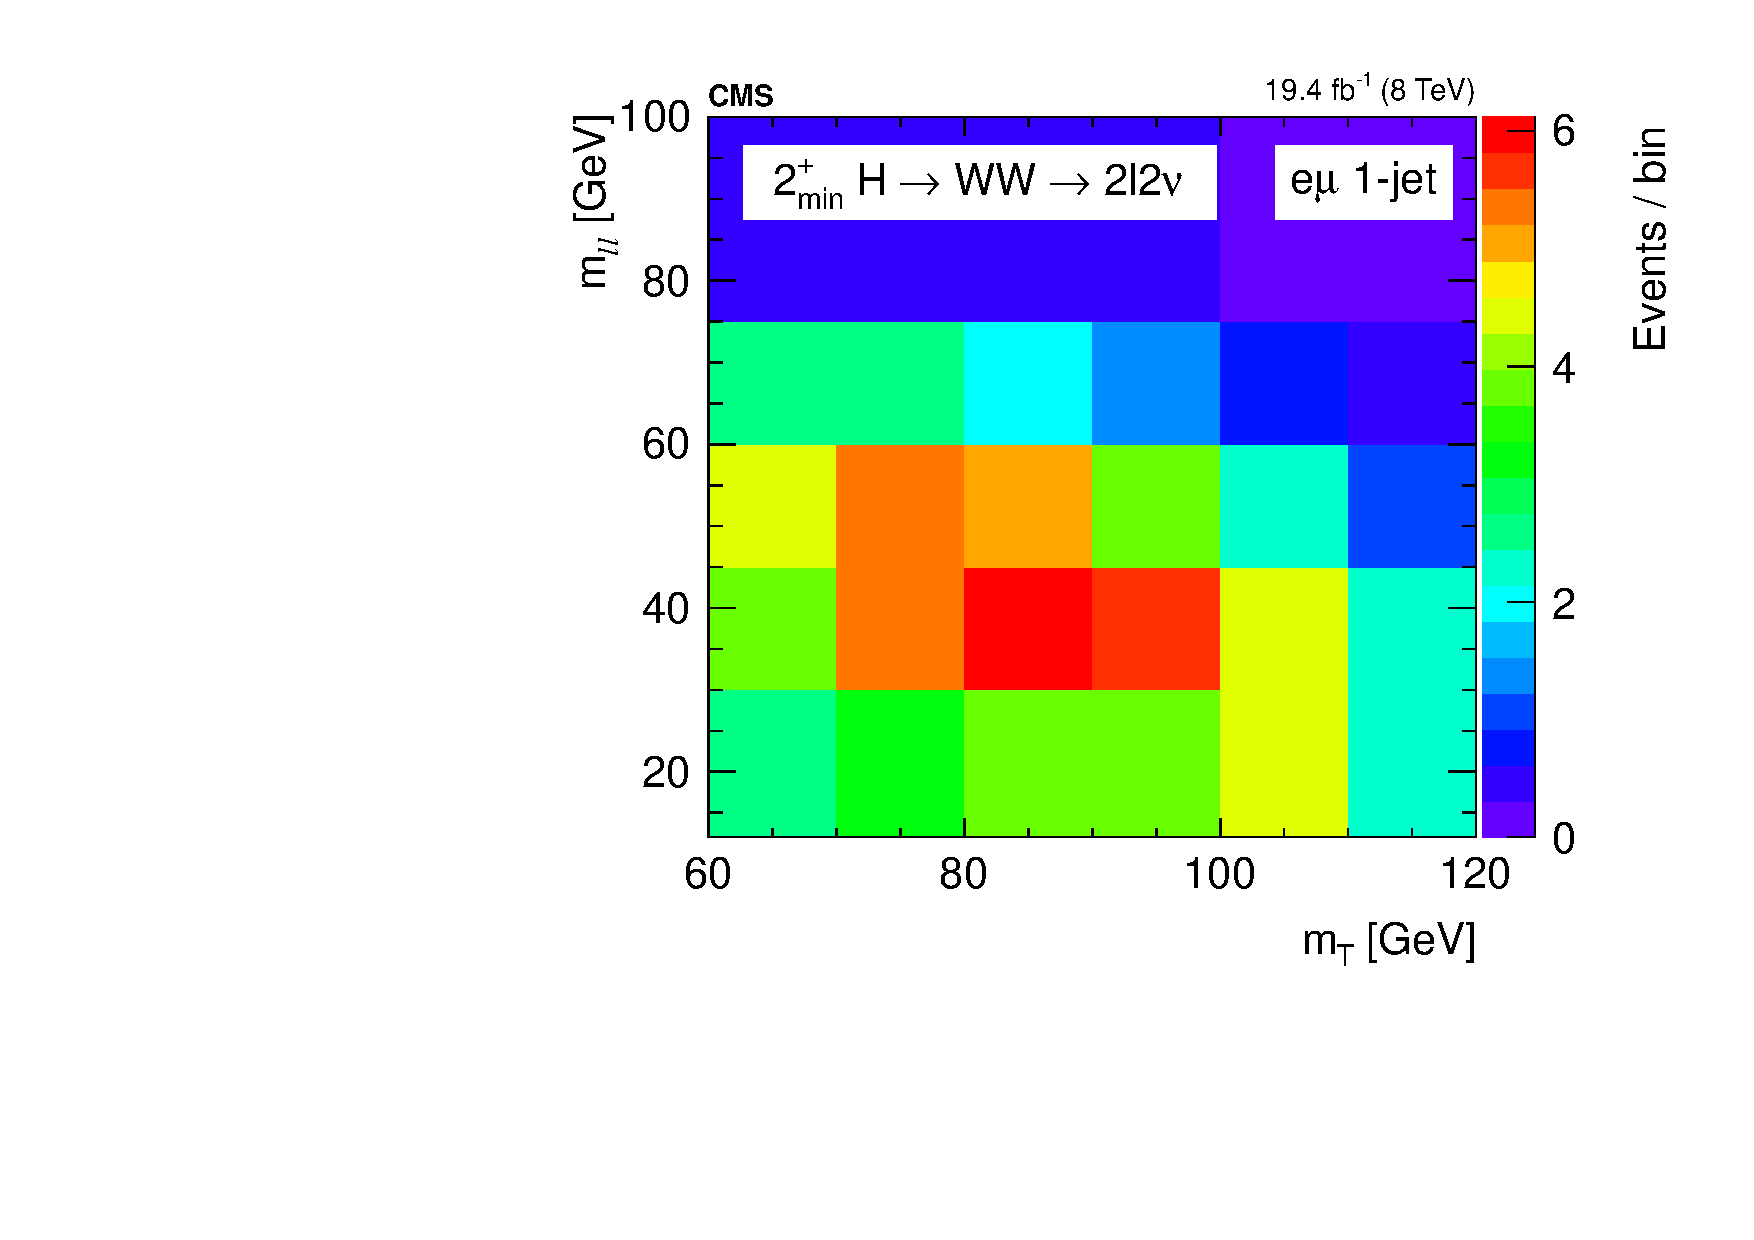
\includegraphics[width=0.45\textwidth]{figures/2d_prefit_1j_125_spin2_paper.pdf}
\caption{2-dimensional templates for $0^+$, $0^-$ and $2_{min}^+$ models.} 
\label{fig:2dtemplates_spin} 
\end{figure} 

Because the $2_{min}^+$ model is generated via $gg\rightarrow X$ and $q\bar{q }\rightarrow X$
modes, and the result depends on the fraction of the two modes. 
We therefore report the results as a function of $q\bar{q} \rightarrow X$ production mode, 
$f_{q\bar{q}}$. Regardless of $f_{q\bar{q}}$, the $2_{min}^+$ model is normalized to the 
SM Higgs cross section. The \qqH\ and \qqVH\ modes are not tested in this study, 
\textit{i.e.} the SM Higgs prediction is used for both hypotheses. 

Fig.~\ref{fig:2dtemplates_spin} shows 2D templates zoomed in the signal region
($60<\mT<120~\GeV$, $0<\mll<100~\GeV$)
for SM Higgs boson, $0^+$  and the $2_{min}^+$ model in 0-jet and 1-jet channels. 
In both channels we clearly see that the $2_{min}^+$ and $0^+$ hypotheses have different shapes 
and we can use this information to discriminate one from the other.
On the other hand, the difference between $0^+$ and $0^-$ 
is not as easily seen as the $2_{min}^+$ case. 
For the backgrounds, the exactly same templates are used as in the 
search analysis. They are shown in fig ~\ref{fig:2dtemplate_125_0j_1}
- \ref{fig:2dtemplate_125_0j_4} for 0-jet. 
\textcolor{red}{what about 1-jet templates?} 

\subsubsection{Test statistic}

For statistical interpretation, we first construct the test statistic($q$). 
It is defined as the difference of the log likelihood between the two 
hypotheses, \textit{i.e.}, alternate model vs. SM Higgs boson. 
\begin{eqnarray} 
q_{alternate} = -2 \ln \mathcal{L}_{alternate} / \mathcal{L}_{0^+}  
\end{eqnarray} 
The likelihood is same as the one used in the SM Higgs search :  
\begin{eqnarray} 
\mathcal{L} ( X | \mu, \theta) 
\, = \,
\prod_{i}^{N_{bin}} \frac{ \left( \mu s_i(\theta) + b_i(\theta) \right)^{X_i}}{X_i!} 
\, e^{ - \mu s_i(\theta) - b_i(\theta) }   \times
\prod_{j}^{N_{nuisance}} p\left( \tilde{\theta_j} | \theta_j \right).
\end{eqnarray}
The only difference in the two likelihoods is the signal component, $s_i$.

We perform a Maximum likelihood fit for each hypothesis with the same dataset 
and the difference in the log-likehood is taken as a statistic. 
In the two fits, the signal strength is allowed to float independently 
and the nuisance parameters in the two models are treated independently. 
The $q$ is calculated using the best-fit values of nuisance parameters. 

The separation is quantified by measuring imcompatility of data with 
the hypothesis under consideration. The expected separation is defined as  
\begin{eqnarray} 
P(q > q_{0^+}^{\textrm{expected}} | \textrm{ alternate model}) 
\end{eqnarray} 
where $q_{0^+}^{\textrm{expected}}$ is the peak position of $q$ assuming $0^+$.
For the observed separation, we can use the observed $q$ from data. 

\section{Results}

Fig.~\ref{fig:llr_spin2} shows the distribution of $q_{2_{min}^+}$ with full data 
combining 0-jet and 1-jet categories. Blue is the expected distribution assumming 
$q_{2_{min}^+}$ and orange is the expected distribution assumming $0^+$ hypothesis.
Top plots show the result with $f_{q\bar{q}}=0~\%$ and the bottom plots show 
the result with $f_{q\bar{q}}=100~\%$. The left plots show the result using the 
expected signal signal strength, $\mu=1$, 
and the right plots show the result using the best-fit value of the signal strength, 
$\mu \approx 0.75$.
Fig.~\ref{fig:llr_band} shows the expected median, $\pm1\sigma$(green) 
and  $\pm2\sigma$(yellow) bands for $q$ assuming $0^+$. 
The blue line is the median of $q$ assuming $2_{min}^+$.
Left is with $\mu=1$ and the right is with observed $\mu$.
Right plot also shows the $q$ calculated using data. 
When the observed $\mu$ is used, the expected separation ranges from 
$1.8\sigma$ to $2.9\sigma$ as $f_{q\bar{q}}$ goes from 0 to 100~\%.
The imcompatibility of data with $2_{min}^+$ model ranges from  
$1.2\sigma$ to $3.1\sigma$ as $f_{q\bar{q}}$ goes from 0 to 100~\%.
We can express this result in terms of \CLs. \CLs\ ranges from 
16.3~\% to 0.2~\% as $f_{q\bar{q}}$ goes from 0 to 100~\%.
All these result shows that data prefers $0^+$ to $2_{min}^+$ hypothesis.  

Fig.~\ref{fig:llr_spin0m} shows the distribution of $q_{0^+}$ with full data 
combining 0-jet and 1-jet categories. When the observed $\mu$ is used, 
The expected(observed) separation 
is $1.2\sigma$($0.8\sigma$) yielding the \CLs=34.7~\%. 
As seen in the 2-dimensional templates in fig.~\ref{fig:2dtemplates_spin},
the sensitivity of separation between $0^+$ and $0^-$ is 
not as good as the $2_{min}^+$ case.

%
\begin{figure}[ht!] 
\centering 
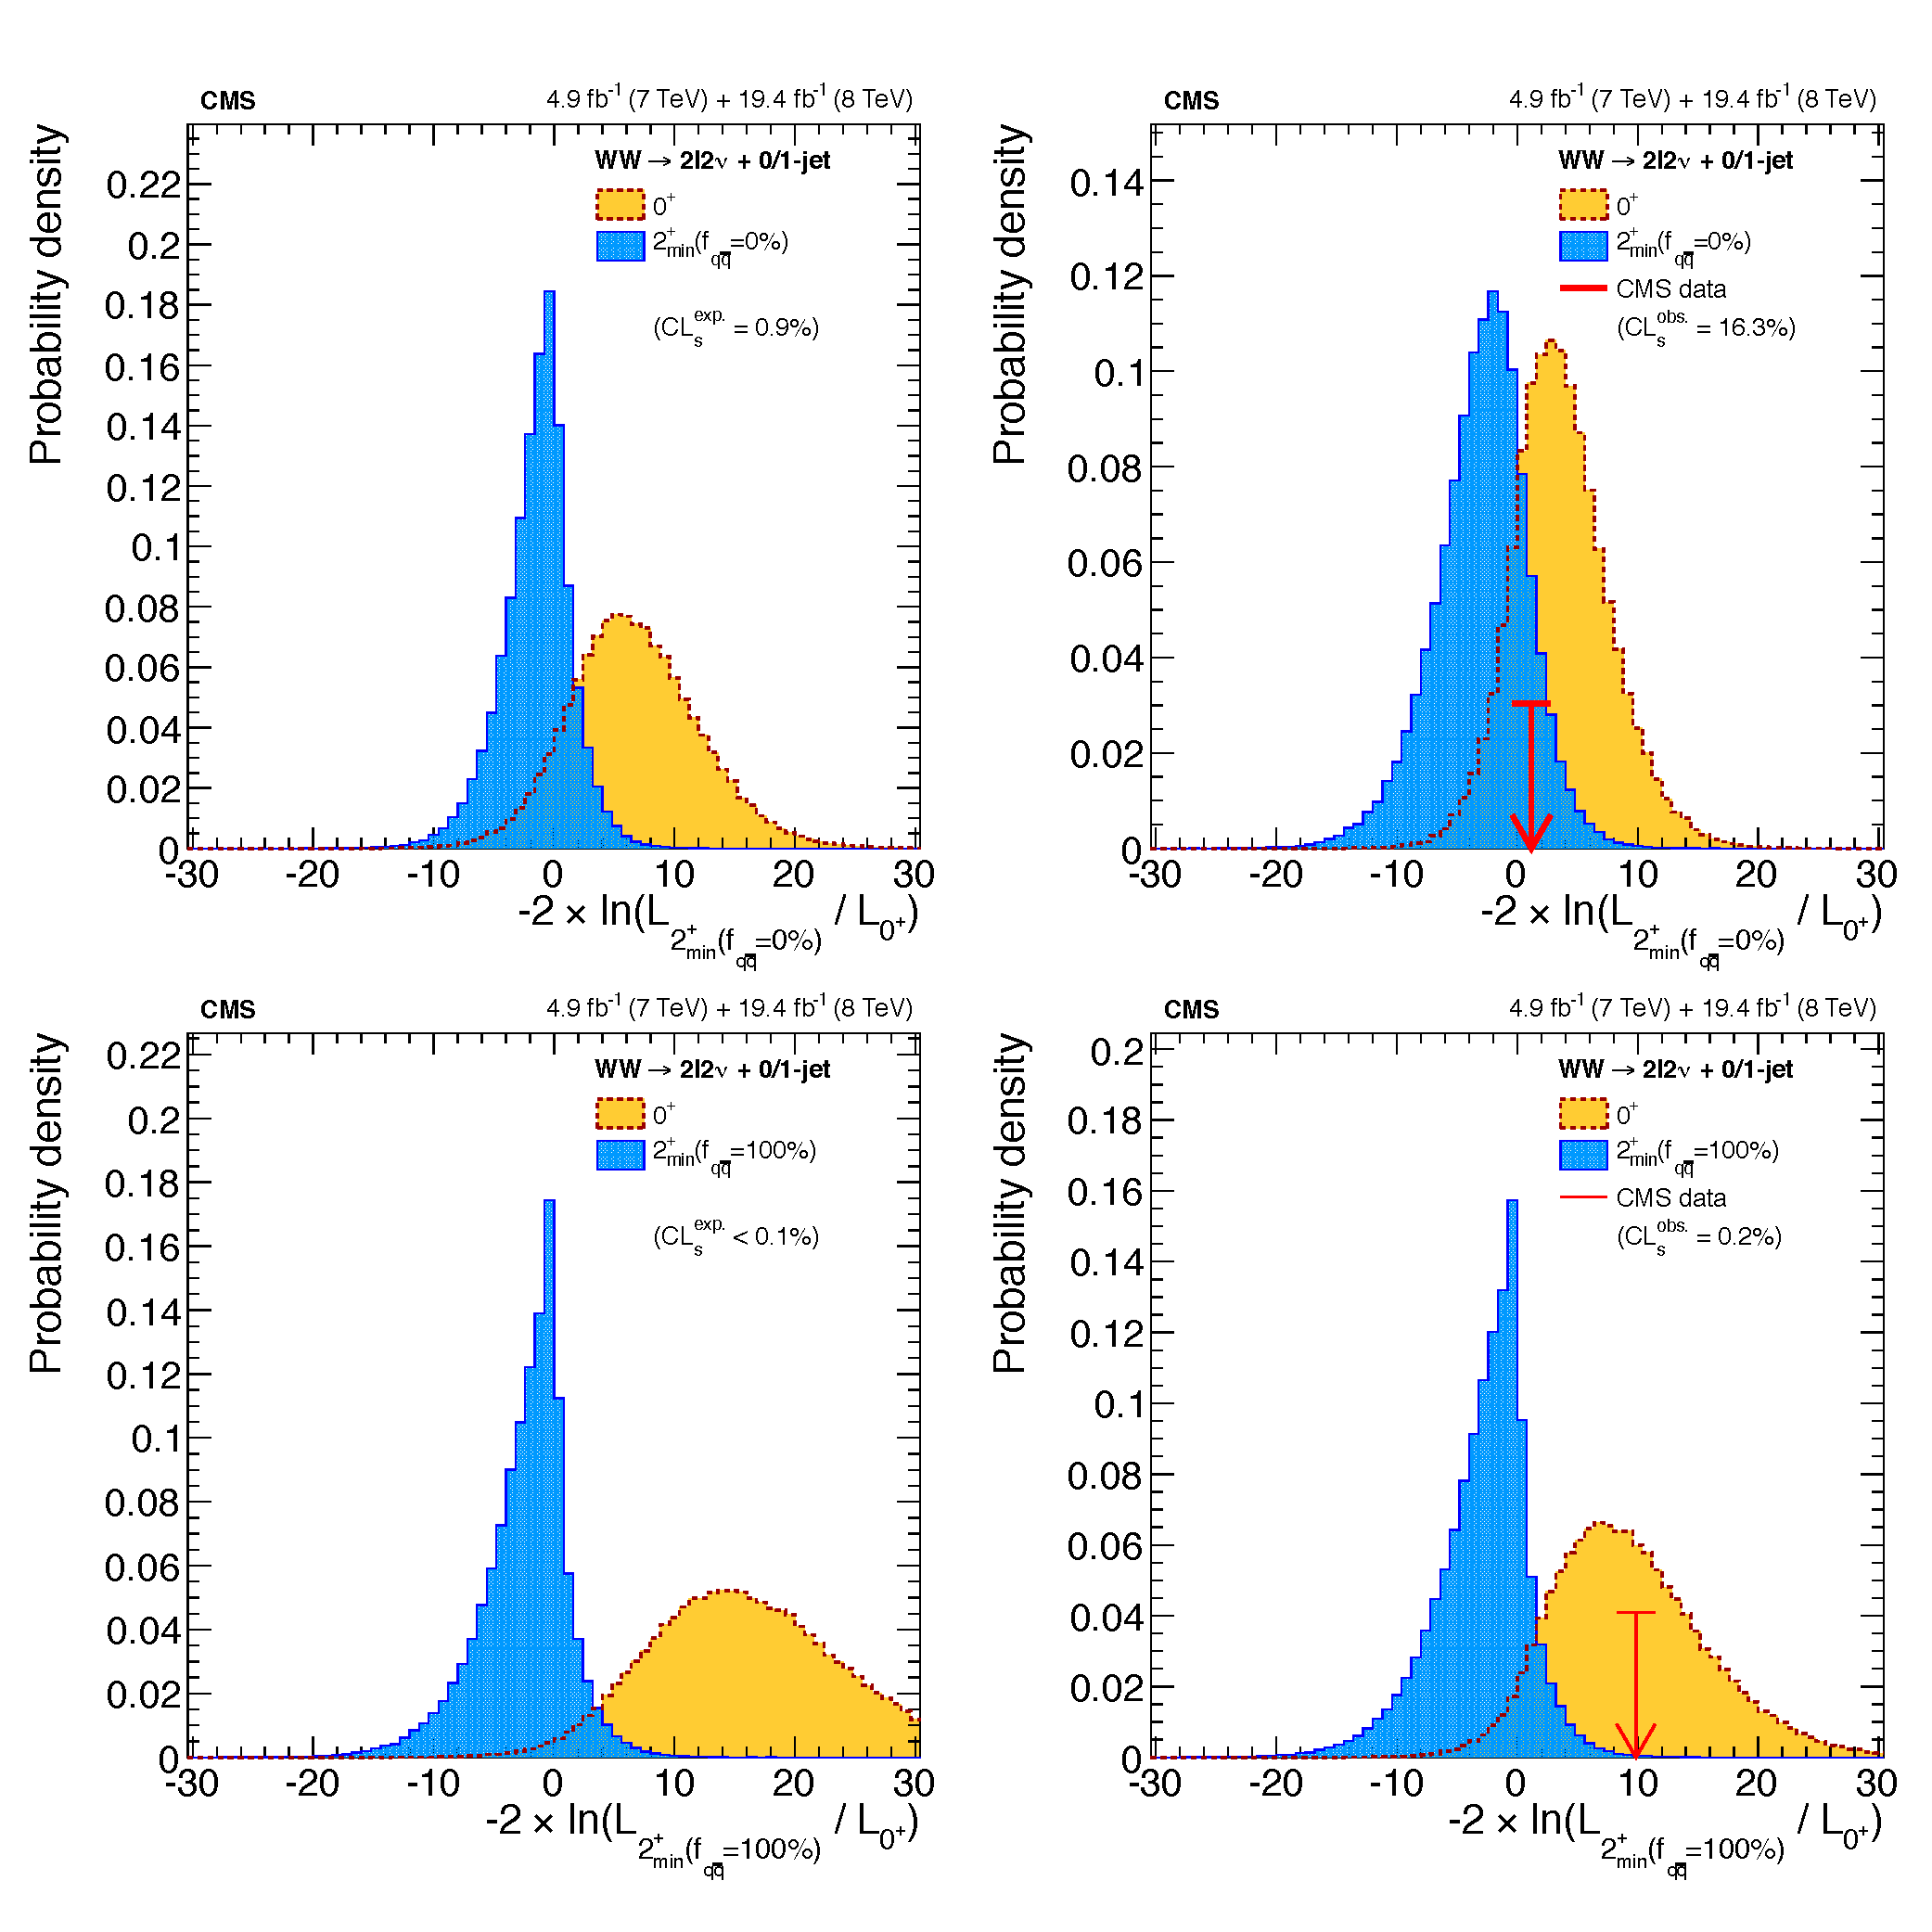
\includegraphics[width=0.9\textwidth]{figures/spin2LLR.pdf}
\caption{Distributions of LLR for spin2}  
\label{fig:llr_spin2} 
\end{figure} 
%
\begin{figure}[ht!] 
\centering 
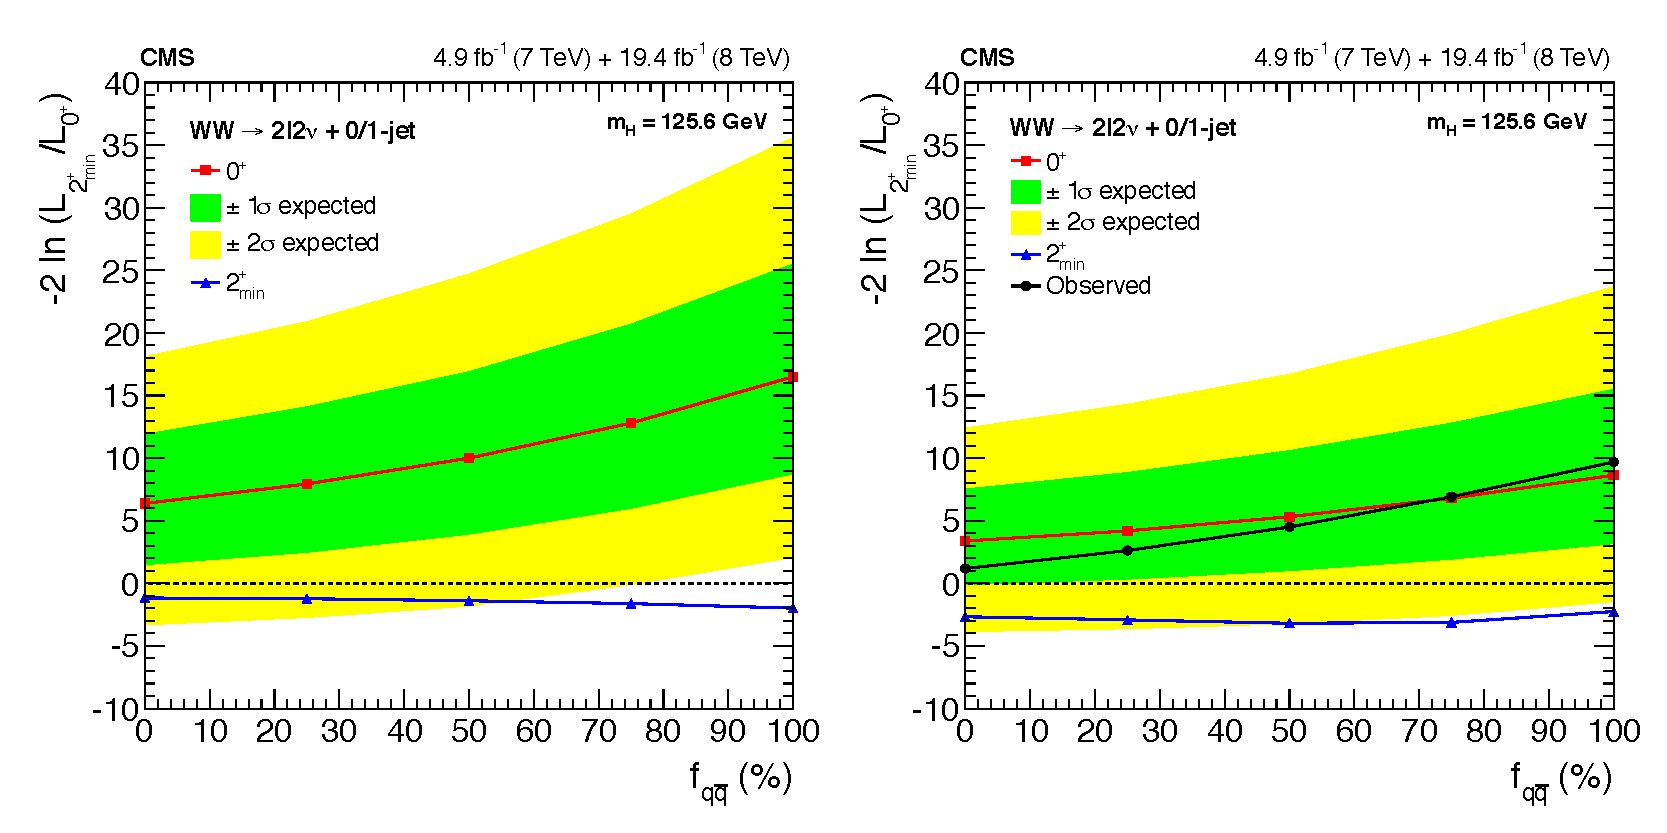
\includegraphics[width=0.9\textwidth]{figures/spinLLRband.pdf}
\caption{Median test static} 
\label{fig:llr_band} 
\end{figure} 
%
\begin{figure}[ht!] 
\centering 
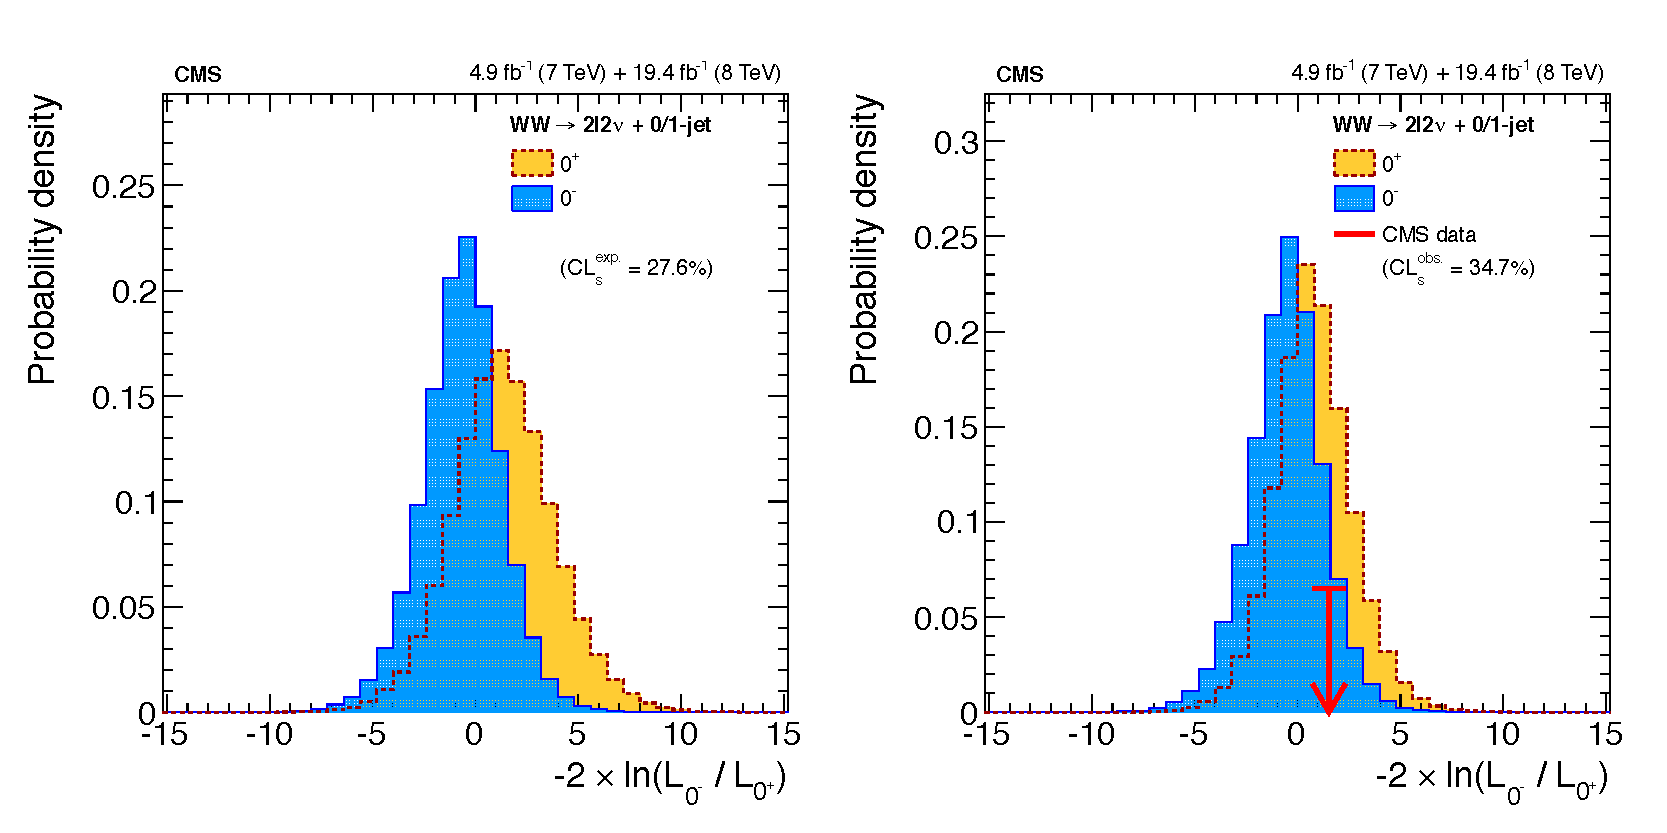
\includegraphics[width=0.9\textwidth]{figures/spin0mLLR.pdf}
\caption{Distributions of LLR for spin0m}  
\label{fig:llr_spin0m} 
\end{figure} 

\section{Conclusion of spin-parity study} 

The spin-parity nature of the new boson is performed against two alternate 
models, $2_{min}^+$ and $0^-$. The result shows that data favors $0^+$ to 
$2_{min}^+$ with \CLs=0.2-16.3\% depending on the fraction of 
$q\bar{q}\rightarrow X$ mode. The \CLs\ with $0^-$ model is 34.7 \%.  


